% \documentclass[conference]{IEEEtran}
\documentclass[12pt,conference]{IEEEtran}
\IEEEoverridecommandlockouts
% The preceding line is only needed to identify funding in the first footnote. If that is unneeded, please comment it out.
\usepackage{cite}
\usepackage{amsmath,amssymb,amsfonts}
\usepackage{algorithmic}
\usepackage{graphicx}
\usepackage{textcomp}
\usepackage{hyperref}
\usepackage{xcolor}
\usepackage{placeins}
\linespread{1.3}
\def\BibTeX{{\rm B\kern-.05em{\sc i\kern-.025em b}\kern-.08em
    T\kern-.1667em\lower.7ex\hbox{E}\kern-.125emX}}
\begin{document}

\title{Predicting Spotify's Next Top Hits}

\author{\IEEEauthorblockN{Elisabetta Caldesi}
\IEEEauthorblockA{\textit{University of Notre Dame} \\
Notre Dame, IN \\
ecaldesi@nd.edu}
\and
\IEEEauthorblockN{Abraham Leon}
\IEEEauthorblockA{\textit{University of Notre Dame} \\
Notre Dame, IN \\
jleon4@nd.edu}
\and
\IEEEauthorblockN{Leigh Campbell}
\IEEEauthorblockA{\textit{University of Notre Dame} \\
Notre Dame, IN \\
lcampbe3@nd.edu}
\and
}

\maketitle


\begin{abstract}
Approximately 51 million people in the U.S. subscribe to music streaming services, a two-fold increase since 2016. Therefore, the increasing popularity of music streaming demands an increasing amount of tailored, fresh content for users. Recently, several companies like the Finnish startup, Hyperlive, claim to predict whether a song will be a hit or not based on its “audio signature”. However, we propose using social sensing to identify songs that will eventually become popular. This is the final paper for \textit{Predicting Spotify's Next Top Hits}, a tool that we have built to predict which new released songs on Spotify will become the next Top Hits based on twitter data. This paper details the impetus and goal of the project, data collection systems, solutions, evaluations, and limitations.
\end{abstract}


\section{Introduction}
Spotify is a digital music and audio streaming service. There are approximately 191 million monthly active Spotify users globally. Moreover, Spotify accounts for 36 percent of the global streaming market, and boasted a quarterly revenue in Q3 2018 at 1.5 billion dollars [1]. Alternatively, Twitter is a popular microblogging platform with reportedly 321 million active monthly users [2]. 
\begin{figure}[h!]
  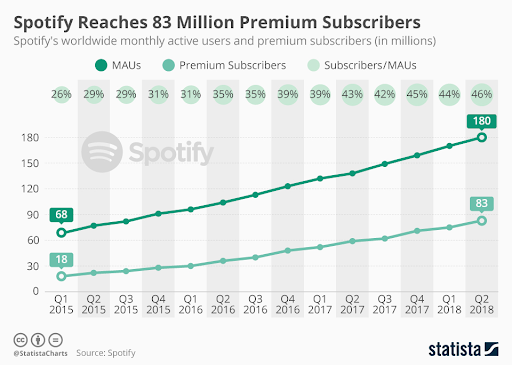
\includegraphics[scale=0.48]{unnamed.png}
  \caption{Number of Spotify Users}
  \label{fig:birds}
\end{figure}
\begin{figure}[h!]
  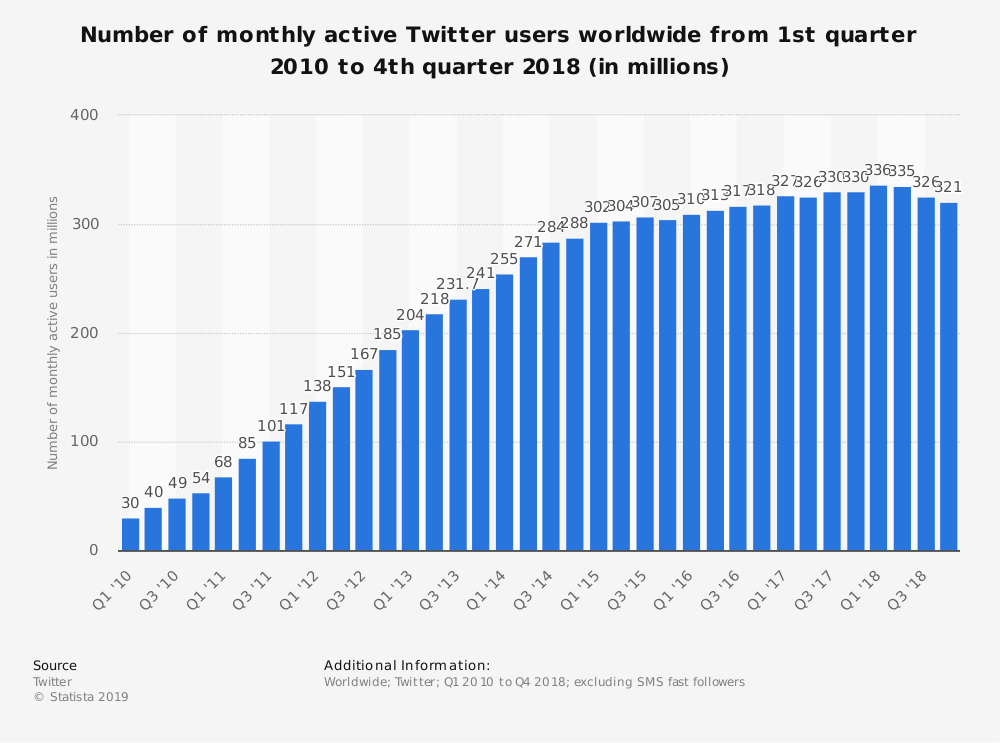
\includegraphics[scale=0.25]{twitter.png}
  \caption{Number of Twitter Users}
  \label{fig:birds}
\end{figure}

The large scope of both these platforms creates a rich and relatively unexplored platform for understanding music popularity. Thus, we developed a straightforward tool to scrape Twitter data and accurately predict the popularity of newly released songs on Spotify using Python libraries Tweepy, GetOldTweets, Spotipy, and Sklearn. We observed strong, linear relationships between topic-frequency related Twitter data and the Spotify popularity index of songs (a combination of how many plays a track has received and how recent those plays were on a scale of 0-100). A multiple linear regression model was generated and evaluated. A schematic of the project design can be seen in Figure 3. \par

\begin{figure}[h!]
  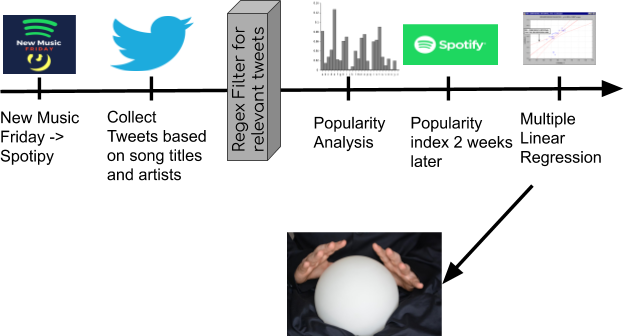
\includegraphics[scale=0.40]{design.png}
  \caption{Project Design}
  \label{fig:birds}
\end{figure}

Despite some limitations, the findings in this project suggest a viable way to predict music streaming popularity. This tool may be valuable for the music industry and personal use. Ultimately, it may also suggest a paradigm that can expanded to other areas of interest like product popularity. This paper will detail this project's methodology, model, results, evaluations, limitations, and future directions. \par

\section{Related Work}
The rise of online social networks and mobile computing has fostered a data-rich environment and tool for mining purposes [2, 3, 4]. Moreover, the use of sensors (and humans as sensors) has transformed this data-rich environment into “context-aware” computing [5]. Social sensing is an emerging field that enables the integration of humans, social networks, and sensors. Twitter, a microblogging social network platform, has been used in numerous social sensing studies. For instance, researchers used Twitter as a real time earthquake detector, and another study evaluated Twitter as a public opinion poller [6, 7]. One previous study also used Twitter to build a predictive model to forecast Billboard music rankings [8]. Nevertheless, there are few studies linking Twitter predictions to Spotify, a popular online music streaming service. \par

\section{Problem Statement}
The primary problem this project seeks to elucidate overlap between the digital platforms Twitter and Spotify. We hope to determine if Twitter data correlates with Spotify song popularity. If so, how can this pattern be quantified and leveraged to predict future song popularity? Moreover, is it possible to create a reliable prediction model based on unreliable data? We believe that the success of this project could greatly help the music industry in determining the next top hit songs before the charts, giving it a chance to discover new talents and songs before everyone else. Overall, this tool can help save money and time thanks to the advantages of using social sensing instead of polls or charts, as Twitter data comes in huge quantities, is readily available, public and represents a wide range of the population. \par

\section{Solution}
In order to train our multiple regression linear model to predict a song's Spotify popularity, we fetched 39 song titles with SPI's between 6 and 99 and their date of release, using the Python library ``Spotipy'' for the Spotify Web API. When choosing the songs, we made sure that they were recent (between mid 2018 and January 2019) but with an established SPI, that hadn't changed in a while. Retrieving the right songs was a difficult task, but we noticed that with a wider SPI range and more current songs our model performed better. Below are the songs from the playlist created for our model training set:
\begin{enumerate}
    \item Tea Gambler                     
    \item Colorblind Mind                 
    \item Nebula Aerobics                 
    \item Nomad Frays                     
    \item Isle Of Strawberries            
    \item Little Piece of Nothing         
    \item No Name No Face                 
    \item Norfolk Drive                   
    \item Cacti for Clothes               
    \item Trouble Always Finds Me         
    \item Even in the Tremor              
    \item Blue Suede Couch                
    \item Cardboard Heart                 
    \item Artificial Paradise             
    \item Lavender Bones                  
    \item Honky Tonk Time Machine         
    \item Do Si Do                        
    \item YNW Home Invasion               
    \item God And Country Music           
    \item Welcome to Silvertown           
    \item Servin Killa Kam                
    \item Walker Texas Ranger             
    \item Shrike                          
    \item Locationships                   
    \item Old Town Road                   
    \item Confessions of a Dangerous Mind 
    \item Splashin                        
    \item Numb Numb Juice                 
    \item Undrunk                         
    \item ilomilo                         
    \item Faucet Failure                  
    \item Mo Bamba                        
    \item wish you were gay               
    \item Thotiana                        
    \item SICKO MODE                      
    \item Let Me Down Slowly              
    \item Murder On My Mind               
    \item Sweet but Psycho                
    \item 7 rings                         
\end{enumerate}

The Spotify popularity index is a combination of how many plays a track has received and how recent those plays were on a scale of 0-100. Therefore, it is a measure of a song's current popularity among Spotify's millions of users. This value is used as our ground truth to determine a song’s popularity. Next, we used the Python library ``GetOldTweets'' to procure a maximum of 4,000 tweets related to the songs since the day of their release. Old Tweets is a useful library because using the Twitter API one can only fetch tweets one week old. Our model could not have been built if we had used the Twitter API live stream since we focused on retrieving tweets as old as August 2018, which was when some of our oldest training set songs were released. Even though the library ``GetOldTweets'' let us filter through the use of keywords for an exact match, we additionally cleaned the tweets and filtered for only content containing the song title or artist using regular expressions matching for artist and song title in different combinations. Through this process, we obtained very clean data to the expense of cutting off some relevant tweets. However, removing relevant tweets wasn't an issue because we retrieved enough tweets to afford losing some relevant ones. \par

Next, we completed sentiment analysis on the Tweets for each song using the Python library ``TextBlob''. This library allowed us to get a value of sentiment for each tweet based on the words that the tweet contained. It gave us a value between -1 and +1. In this model, a negative value represents a negative sentiment in a tweet, while a positive value represents a positive sentiment. For each song, we also noted the total number of filtered tweets collected, the time it took to search the tweets, the total number of favorites and the total number of retweets both as sums of the favorites and the retweets of each tweet that passed our filters. These volume related variables give an indication of ``audience-reached''. \par

In order to determine which were the relevant variables for the model, we calculated the Pearson correlation between these variables and the song SPI. The Pearson correlation shows the linear relationship between the variable and the SPI, a value close to 0 represents weak correlation, while a value close to 1 represents strong correlation. After we determined the Pearson correlation values for each variable, we proceeded to calculate the R-squared value for the relationship between the variable and the SPI, to determine which mathematical model would fit the relationship best. Following linear validation with Pearson correlations and R-squared model fitting, a multiple linear regression model with the Python library ``Sklearn'' where the Twitter data was used as independent variables and the Spotify popularity index as the dependent variable.\par 

Finally, to test this model, we created a Twitter bot using the Python library ``Tweepy'' that scrapes data filtered by the keywords generated from the song titles and artists retrieved from the Spotify playlist ``New Releases Friday''. The tweets collected from this playlist were also filtered using the regex functions that we implemented and the basic filter that removes links, usernames and other text that might interfere with results. Using the multiple linear regression model coefficients, the predicted SPI of each song was calculated. Two weeks later, the actual Spotify SPI was fetched and the accuracy of calculation assessed.  \par

\section{Evaluation}
To create a model for predicting SPI, 40 songs with SPI’s between 6 and 99 were fetched from Spotify. The songs and the Twitter data collected for each can be seen below. \par


% \begin{table}[htb]
%   \centering
%     \caption{Training Set Results}
%     \tabcolsep=0.11cm
\begin{center}
\begin{small}
{\begin{tabular}{l|l|l|l}
\centering 
\textbf{Song} & \textbf{Tweets} & \textbf{Favorites} & \textbf{Rts}      \\
Tea Gambler                     & 2      & 8         & 6        \\
Colorblind Mind                 & 6      & 17        & 1        \\
Nebula Aerobics                 & 6      & 11        & 2        \\
Nomad Frays                     & 5      & 4         & 2        \\
Isle Of Strawberries            & 15     & 26        & 8        \\
Little Piece of Nothing         & 31     & 25        & 1        \\
No Name No Face                 & 16     & 36        & 7        \\
Norfolk Drive                   & 17     & 47        & 11       \\
Cacti for Clothes               & 25     & 2         & 0        \\
Trouble Always Finds Me         & 93     & 121       & 30       \\
Even in the Tremor              & 131    & 1230      & 212      \\
Blue Suede Couch                & 38     & 195       & 22       \\
Cardboard Heart                 & 100    & 1618      & 200      \\
Artificial Paradise             & 104    & 289       & 90       \\
Lavender Bones                  & 89     & 388       & 38       \\
Honky Tonk Time Machine         & 245    & 5034      & 857      \\
Do Si Do                        & 71     & 120       & 4        \\
YNW Home Invasion               & 103    & 84        & 14       \\
God And Country Music           & 38     & 188       & 69       \\
Welcome to Silvertown           & 70     & 229       & 100      \\
Servin Killa Kam                & 887    & 1003      & 326      \\
Walker Texas Ranger             & 1505   & 4055      & 865      \\
Shrike                          & 1500   & 10749     & 1302     \\
Locationships                   & 1934   & 7740      & 1004     \\
Old Town Road                   & 3950   & 79273     & 9378     \\
Confessions of a Dangerous Mind & 1793   & 43756     & 9710     \\
Splashin                        & 2952   & 16333     & 3077     
\end{tabular}}
\end{small}
\end{center}

\begin{center}
\begin{small}
{\begin{tabular}{l|l|l|l}
\centering
Numb Numb Juice                 & 2728   & 13751     & 2841     \\
Undrunk                         & 3263   & 53777     & 5406     \\
ilomilo                         & 2381   & 11160     & 1130     \\
Faucet Failure                  & 2807   & 61099     & 7189     \\
Mo Bamba                        & 2922   & 31005     & 3727     \\
wish you were gay               & 1711   & 10999     & 1402     \\
Thotiana                        & 3750   & 264027    & 72691    \\
SICKO MODE                      & 2840   & 56205     & 8283     \\
Let Me Down Slowly              & 3627   & 15080     & 2292     \\
Murder On My Mind               & 3379   & 29571     & 5263     \\
Sweet but Psycho                & 2476   & 12061     & 1623     \\
7 rings                         & 2093   & 84576     & 21781   
\end{tabular}}
\end{small}
\end{center}

\begin{center}
\begin{small}
{\begin{tabular}{l|l|l}
\centering
\textbf{Song}                   & \textbf{Time (ms)}   & \textbf{Sentiment}    \\
Tea Gambler                     & 1.722 & 0.125        \\
Colorblind Mind                 & 10.402 & 0.14961  \\
Nebula Aerobics                 & 50.301 & 0.08720  \\
Nomad Frays                     & 30.400 & 0.02727  \\
Isle Of Strawberries            & 92.104 & 0.11593  \\
Little Piece of Nothing         & 45.325 & -0.08645 \\
No Name No Face                 & 27.428 & -0.06399 \\
Norfolk Drive                   & 13.835 & 0.10487  \\
Cacti for Clothes               & 71.080 & 0.03743  \\
Trouble Always Finds Me         & 1282.404 & -0.09058 \\
Even in the Tremor              & 2529.377 & 0.07867  \\
Blue Suede Couch                & 517.389  & 0.103    \\
Cardboard Heart                 & 210.694 & 0.03265  \\
Artificial Paradise             & 2113.585 & -0.31938 \\
Lavender Bones                  & 90.375 & 0.060908 \\
Honky Tonk Time Machine         & 4373.929 & 0.148810 \\
Do Si Do                        & 525.363 & 0.080399 \\
YNW Home Invasion               & 1606.668 & 0.094105 \\
God And Country Music           & 367.052 & 0.131143 \\
Welcome to Silvertown           & 1001.745 & 0.504666 \\
Servin Killa Kam                & 11358.750 & 0.061704 \\
Walker Texas Ranger             & 20192.110 & 0.066553 \\
Shrike                          & 12677.050 & 0.139252 \\
Locationships                   & 43523.760 & 0.128736 \\
Old Town Road                   & 99968.330 & 0.095087 \\
Confessions of a Dangerous Mind & 45012.831 & -0.40473 \\
Splashin                        & 49487.457 & 0.152540  \\
Numb Numb Juice                 & 38836.603 & -0.46812 \\
Undrunk                         & 69047.196 & 0.070403  
\end{tabular}}
\end{small}
\end{center}

\begin{center}
\begin{small}
{\begin{tabular}{l|l|l}
\centering
ilomilo                         & 38305.182   & 0.124432924  \\
Faucet Failure                  & 48712.506 & -0.176340978 \\
Mo Bamba                        & 54383.032  & 0.061640232  \\
wish you were gay               & 31350.062  & 0.293964837  \\
Thotiana                        & 75756.953 & -0.007733083 \\
SICKO MODE                      & 45068.658 & 0.047411372  \\
Let Me Down Slowly              & 81470.863 & -0.194908493 \\
Murder On My Mind               & 81012.883 & 0.020493285  \\
Sweet but Psycho                & 36017.491 & 0.310041377  \\
7 rings                         & 25479.452 & 0.068322692 
\end{tabular}}
\end{small}
\end{center}

To determine the relationship between the independent Twitter variables and SPI, each variable was plotted against SPI and the R-squared values for trend lines calculated and the Pearson correlation coefficients calculated. The variables of search time, number of tweets, number of retweets, and number of favorites all had strong logarithmic relationship to SPI as seen in the Figures 4, 5, 6 and 7.

\begin{figure}[h!]
  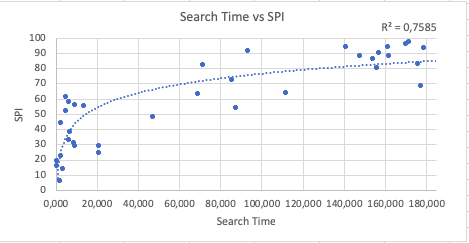
\includegraphics[scale=0.5]{search.png}
  \caption{SPI vs Search Time}
  \label{fig:birds}
\end{figure}

\begin{figure}[h!]
  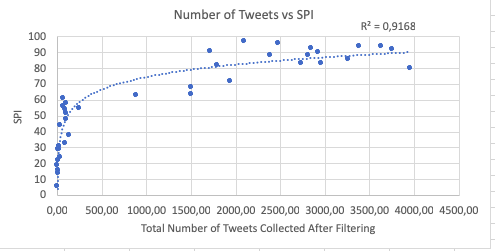
\includegraphics[scale=0.5]{number.png}
  \caption{SPI vs Number of Tweets}
  \label{fig:birds}
\end{figure}

\begin{figure}[h!]
  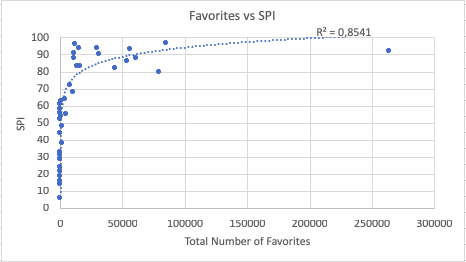
\includegraphics[scale=0.5]{favs.png}
  \caption{SPI vs Number of Favorites}
  \label{fig:birds}
\end{figure}

\begin{figure}[h!]
  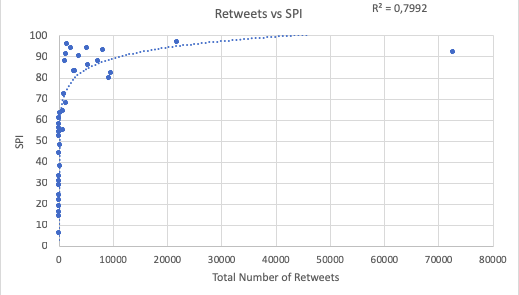
\includegraphics[scale=0.48]{rts.png}
  \caption{SPI vs Number of Retweets}
  \label{fig:birds}
\end{figure}

Upon inspection, logarithmic relationships were logical because the SPI is limited to 100 while the twitter data can be theoretically unlimited. The Pearson correlation coefficients also demonstrated strong, positive linear correlations between variables and SPI. The Pearson correlation coefficient for the logarithms of the number of tweets, the total number of favorites, the total number of retweets, and the search time to SPI are shown in Table I. These values suggest that a multiple linear regression may be a strong model in predicting SPI. Based on this analysis, we used the Python library ``Sklearn'' to build our multiple linear regression model to calculate the coefficients.

\begin{table}[htb!]
\centering
\caption{Pearson Correlation Coefficients}
{\begin{tabular}{l|l}
Variable                    & Pearson Correlation  \\
Total number of tweets      & 0.9575053             \\
Total number of favorites   & 0.92417781            \\
Total number of retweets    & 0.89396239            \\
Search time                 & 0.87089819
\end{tabular}}
\end{table}

\begin{equation}\label{my_first_eqn}
        SIP = \beta_{0} + \beta_{1}(t) + \beta_{2}(f) + \beta_{3}(r) + \beta_{4}(n)
\end{equation}

The variables in Equation (1) represent the following: SIP is the Spotify Popularity Index, t is the log of time it took to search, f is the log of the total number of favorites, r is the log of total number of retweets and n is the log of the number of filtered tweets collected. SIP is the dependent variable of our model while t, f, rts and n are the independent variables. $\beta{_1}$, $\beta{_2}$, $\beta{_3}$, $\beta{_4}$ are the regression coefficients which represent the importance of our independent variables in our model and $\beta{_0}$ is the interception value. Table II shows the values of the calculated weights.

\begin{table}[htb!]
 \centering
  \caption{Regression Coefficient Values}
{\begin{tabular}{l|l}
Coefficient & Value \\
$\beta{_0}$ & $-3,3357688$ \\
$\beta{_1}$ & $22,6259999$ \\
$\beta{_2}$ & $3,31975537$ \\
$\beta{_3}$ & $-0,1487848$ \\
$\beta{_4}$ & $-1,1325846$ \\
\end{tabular}}
\end{table}

The final equation for our multiple linear regression model is: \newline
$SIP$ $=$ $-3,3357688$ $+$ $22,6259999(t)$ $+$ $3,31975537(f)$ $-$ $0,1487848(r)$ $-$ $1,1325846(n)$

Every Friday, we retrieved from the Spotify playlist ``New Music Friday''. Over the course of two weeks, we collected 4,000 tweets per song to compute the variables necessary for the multiple linear regression at the end of the two weeks. We tested our model on 300 songs and were able to predict the Spotify Popularity Index with an error of 11,67459776. Upon further inspection, we noticed that some of our predictions were not as accurate as the average predictions. By analyzing the tweet content that we were fetching, we realized that Twitter bots negatively affect our predictions. This is because on Twitter there are many accounts that act as bots, which retweet some tweets many times. Since our model does account for the total number of retweets found, it is very sensitive to Twitter bots. Therefore, our project acts as a Twitter bot detector, because it evaluates the song SPI with very low accuracy, usually between 0 and 30 per cent. When removing those songs that can be considered outliers since they were affected by bots, our prediction error is reduced to 7,231176445. Overall we can say that our model predicts the SPI with strong accuracy and relatively low error.


\section{Discussion and Limitations}
Despite a clear and strong relationship between twitter data and SPI, it is worth noting the several limitations of this project. First, it was necessary to apply stringent filters to Twitter data to obtain clean data. Twitter’s API filter keyword feature performs an exact match on tweets including the exact keywords that are specified. As stated by the API’s documentation “a phrase will match if all of the terms in the phrase are present in the Tweet, regardless of order and ignoring case.” Hence, having a keyword that is a common everyday word as one of the keywords would yield problematic results. Song titles with routine names generate irrelevant Twitter data. For instance, the song ``Wow'' by Post Malone collects thousands of tweets that use the word ``wow'' not in the context of this song. But adding other keywords such as artist name didn't generate helpful results either because people might not spell out songs with their full titles or followed by their artists, but the Twitter Streaming API searches for exact matches of our keywords. \par

To address this issue, we created additional regex filter functions after collecting tweets. This regex requires a tweet to specifically include an artist and a song title in different combinations or only the song title. This by no means is a perfect filter. At the expense of the number of tweets that pass the filter, the data is more credible and useful. Below, Table III and IV are examples of tweets before and after our filter for the song ``7 rings'' by Ariana Grande and ``Stay Flo'' by Solange: 

\begin{table}[htb!]
 \centering
  \caption{7 Rings Collected Filtered Tweets}
{\begin{tabular}{c}
im eating at good pho you and they're playing 7 rings. 5 stars. \\
back at number 1 again. 7 rings just won't let up.. \\
7 rings is the song i’m the most excited to see her perform \\
7 rings is back at no. 1 where it belongs \\
7 rings for the first time live! \\
7 rings not even that good of a song to be no.1 in the country \\
you like the worst song of all time aka 7 rings. \\
\end{tabular}}
\end{table}

\begin{table}[htb!]
 \centering
  \caption{Stay Flo Collected Filtered Tweets}
{\begin{tabular}{c}
stay flo is the best song on when i get home. \\
no idea what solange is talking about on stay flo but i love it \\
i listened to solange stay flo 700 times this week \\
this is what makes stay flo the best song from when i get home \\
stay flo stuck in my head again and i do not mind at all \\
stay flo by solange is how i like to start my morning \\
stay flo by solange is just that song for me rn \\

\end{tabular}}
\end{table}

Furthermore, for the sake of more accurate Twitter data collection, we purposefully chose songs that had non-conversational titles for our training set and testing songs. This limited the ability of the tool predict the popularity of some songs. \par

Additionally, sentiment analysis unexpectedly proved to be irrelevant in this project. The accuracy of TextBlob's sentiment analysis was poor. We have noted that TextBlob is not particularly applicable to the vernacular of microblogging. For instance, TextBlob coded slang sayings like ``on point'' (a positive sentiment) as ``neutral''. The polarity of sentiment seemed to be random at times. Song titles with sentiments within them also need to be removed from tweets because they could influence sentiment analysis scoring. An example of this are the songs ``Bad Liar'' by Imagine Dragons or ``Sweet but Psycho'' by Ava Max which contain ``Bad'' and ``Sweet''. As the word has a positive connotation, TextBlob sentiment would seem to yield positive sentiments for the most part regardless of the context of the tweet. \par

\begin{figure}[h!]
  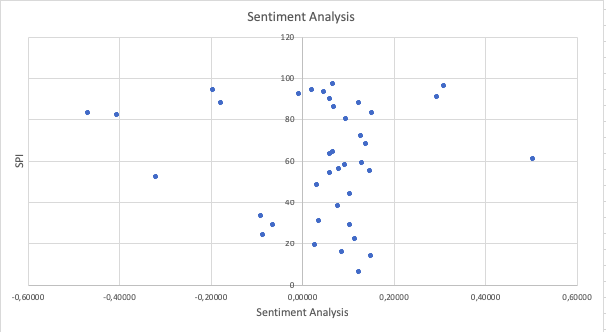
\includegraphics[scale=0.4]{senti.png}
  \caption{SPI vs Average Tweet Sentiment}
  \label{fig:birds}
\end{figure}

As seen in the Figure 8, there was not a clear relationship between average tweet sentiment and SPI. The Pearson correlation coefficient between average sentiment and SPI was -0.07, suggesting an extremely weak, negative relationship. Additionally, in the initial multiple linear model regression sentiment coefficient had a p-value of 0.27. These findings further suggested it was an irrelevant variable in our model, and thus we did not use it. Furthermore, we attempted to create our own sentiment analysis, but could not find a “slang” lexicon large enough and relevant enough to be sufficient for Twitter sentiment analysis. Other tools displayed similar results as TextBlob. The vernacular of Twitter is difficult to analyze with lexicons based on standard English. \par

As mentioned before, we also observed skewed results when Twitter bots repeatedly tweeted about songs. For example, the song “Everybody here hates you” was only predicted with 33 \% accuracy. We observed Twitter bot patterns in data collected inaccurate prediction, including the same tweet tweeted repeatedly by a single account. In the future, this project could be improved by developing or adapting a Twitter bot detector tool. However, this tool could also be expanded as a music bot detector itself. \par

Finally, the time-frame of this project is limited to two-week intervals. This time-frame was chosen in order to collect sufficient amounts of data and it is when we believe SPI stabilizes for a given song. However, this project could be expanded to predict more precise SPI predictions in a shorter time frame, and thus be even more timely for industry use. \par
This project could also be expanded to other industries and not only the music industry, the main expansion required would be to evaluate if the variables that we discovered were relevant for our multiple linear regression model would still apply to other products, but once the variables are fixed the model can be easily trained and developed. 

\section{Conclusion}
The purpose of this project was to create a tool to predict Spotify song popularity based on Twitter data. Using Spotify and Twitter APIs, we created a multiple linear regression model to predict the Spotify Popularity Index of a newly released song based on twitter data relating to the song (number of tweets, retweets, favorites, and time to gather 4,000 tweets). The model predicted song popularity with 93 percent accuracy excluding outliers. Despite this strong, linear correlation between Twitter data and SPI, this project is limited in scope. Due to Twitter filtering, only non-conversational song titles could be used. Additionally, this project is limited to a two-week time frame for predictions. However, taken together these findings suggest Twitter may be a viable tool for forecasting music popularity in streaming services like Spotify. \par

\section{Source Code}
The source code that we created for this study can be found in the following GitHub repository:
\begin{center}
\url{https://github.com/aleon1996/SSProject}
\end{center}
NOTE: This project requires the use of the Twitter and Spotify APIs. In order to run this code to collect tweets or gather music data from Spotify, a developer needs to have access to tokens. For the purpose of privacy, we have removed our personal tokens and API keys from the source code. However, these tokens and IDs can be acquired through the official developer site for Twitter and for Spotify. Information on how to run this code can be found in the project's README.\par

% \clearpage

\section{References}
\begin{enumerate}
    \item http://www.businessofapps.com/data/spotify-statistics/
    \item https://www.washingtonpost.com/technology
    /2019/02/07/twitter-reveals-its-daily-active-
    user-numbers-first-time/
    \item G. Qi, C. Aggarwal, T. Huang. Community Detection with Edge Content in Social Media Networks, ICDE Conference, 2012.
    \item T. Zhang, A. Popescul, B. Dom. Linear prediction models with graph regularization for web-page categorization. In KDD, pages 821–826, 2006.
    \item Y. Zhou, H. Cheng, J. X. Yu. Graph clustering based on structural/attribute similarities. PVLDB, 2(1): pp. 718–729, 2009.
    \item C. Aggarwal, T. Abdelzaher. The Internet of Things: A Survey From the Data-Centric Perspective: Chapter 9 Social Sensing. Springer 2013.
    \item \url{https://www3.nd.edu/~dwang5/courses/spring19/papers/media-sensing/twitter-earthquake.pdf}
    \item \url{https://www3.nd.edu/~dwang5/courses/spring19/papers/media-sensing/tweets-to-polls.pdf}
    \item \url{https://www.researchgate.net/publication/290060220}

\end{enumerate}



\end{document}
